\documentclass[a4paper,12pt,fleqn]{article}
\usepackage{fixltx2e}
\usepackage[utf8]{inputenc}
\usepackage{graphicx}
\usepackage{sidecap}
\usepackage{fancyhdr}
\usepackage{amssymb,amsmath}
\usepackage[swedish]{babel}
\usepackage[margin=1.5in]{geometry}
\usepackage{abstract}
\usepackage[parfill]{parskip}
\usepackage{tocloft}
\usepackage{adjustbox}
\usepackage{textcomp}
\usepackage[T1]{fontenc}
\usepackage[usenames,dvipsnames,svgnames,table]{xcolor}
\usepackage{listings}
\usepackage{hyperref}
\usepackage{tocloft}

% %% Footnotes-Listing %%
\newcommand{\listfootnotesname}{Referenser}% 'List of Footnotes' title 
\newlistof[chapter]{footnotes}{fnt}{\listfootnotesname}% New 'List of...' for footnotes 
\let\oldfootnote\footnote % Save the old \footnote{...} command 
 \renewcommand\footnote[1]{% Redefine the new footnote to also add 'List of Footnote' entries. 
     \refstepcounter{footnotes}% Add and step a reference to the footnote/counter. 
     \oldfootnote{#1}% Make a regular footnote. 
     \addcontentsline{fnt}{footnotes}{\protect 
 \numberline{\thefootnotes}#1}% Add the 'List of...' entry. 
}

%----------------------------------------------------------------
%C-kod formatering

\definecolor{listinggray}{gray}{0.9}
\definecolor{lbcolor}{rgb}{0.9,0.9,0.9}
\lstset{
backgroundcolor=\color{lbcolor},
    tabsize=4,    
%   rulecolor=,
    language=[GNU]C++,
        basicstyle=\scriptsize,
        upquote=true,
        aboveskip={1.5\baselineskip},
        columns=fixed,
        showstringspaces=false,
        extendedchars=false,
        breaklines=true,
        prebreak = \raisebox{0ex}[0ex][0ex]{\ensuremath{\hookleftarrow}},
        frame=single,
        numbers=left,
        showtabs=false,
        showspaces=false,
        showstringspaces=false,
        identifierstyle=\ttfamily,
        keywordstyle=\color[rgb]{0,0,1},
        commentstyle=\color[rgb]{0.026,0.112,0.095},
        stringstyle=\color[rgb]{0.627,0.126,0.941},
        numberstyle=\color[rgb]{0.205, 0.142, 0.73},
%        \lstdefinestyle{C++}{language=C++,style=numbers}’.
}
\lstset{
    backgroundcolor=\color{lbcolor},
    tabsize=4,
  language=C++,
  captionpos=b,
  tabsize=3,
  frame=lines,
  numbers=left,
  numberstyle=\tiny,
  numbersep=5pt,
  breaklines=true,
  showstringspaces=false,
  basicstyle=\footnotesize,
%  identifierstyle=\color{magenta},
  keywordstyle=\color[rgb]{0,0,1},
  commentstyle=\color{Darkgreen},
  stringstyle=\color{red}
  }
  %-----------------------------------------------------------------
  %marginaler

  \renewcommand{\abstractnamefont}{\normalfont\normalsize\bfseries}
  \renewcommand{\abstracttextfont}{\normalfont\small}
  \renewcommand{\headrulewidth}{0pt}
  \renewcommand{\cftsecleader}{\cftdotfill{\cftdotsep}} 
  \setlength{\absleftindent}{0pt}
  \setlength{\absrightindent}{0pt}
  \setlength{\headheight}{15pt}

  \addtolength{\oddsidemargin}{-.5in}
  	\addtolength{\evensidemargin}{-.5in}
  	\addtolength{\textwidth}{1in}


  %-----------------------------------------------------------------
  %header and footer

  \pagestyle{fancy}
  \lhead{
  	\begin{picture}(0,0)
  		\put(5,0){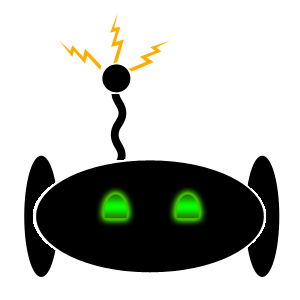
\includegraphics{logotyp.png}}
  	\end{picture}}
	
  \fancyhead[C]{\small{Mapmaster2001}}
  \fancyhead[R]{\small \today}
  \fancyfoot[L]{\small{TSEA56 \\ LIPS Kappa}}
  \fancyfoot[C]{\small{\thepage}}
  \fancyfoot[R]{\small{Projektgrupp 8 \\ mapmaster2001@cyd.liu.se}}

  %-----------------------------------------------------------------


%-------------------------------------------------------------------
%Första sidan

\begin{document}
	\pagestyle{fancy}
\pagenumbering{roman}
	\vspace*{\fill}
		\begingroup
			\begin{center}
				\huge{\textbf{Teknisk dokumentation}}
				\\
				\vspace{5pt}
				\normalsize
				Kandidatprojekt Y - Grupp 8 - VT2014
				\\
				Version 1.0
				\end{center}
		\endgroup
	 
	\vspace{15pt}
	\vspace*{\fill}
	
	\begin{center} %Börjar centrering 
		Status
		\\
		\vspace{3pt} %Whitespace 3 pts
	    \begin{tabular}{| p{3cm} | p{3cm} | p{3cm} |} %tabell, 4 horizontella |, 3 cm emellan dem.
	    \hline %översta horizontella linjen.
	    Granskad & JE,TG,HFE & \today \\ \hline % & -tecken för att "gå till nästa ruta" 
		Godkänd & - & - \\ \hline % avslutas med \\ och \hline.

	    \end{tabular}
	\end{center}
	\vspace{2cm}
	\newpage
%-----------------------------------------------------------------
%Projektidentitet
	
	\vspace*{\fill}
		\begingroup
			\begin{center}
				\LARGE{\textbf{PROJEKTIDENTITET}}
				\\
				\footnotesize
				Grupp 8, 2014/VT, MapMaster2001
				\\
				Linköpings tekniska högskola, ISY
				\\
				\vspace{1cm}
	  \begin{tabular}{| p{3cm} | p{4.3cm} | p{2.4cm} | p{3.8cm} |}
	    \hline
		\textbf{Namn} & \textbf{Ansvar} & \textbf{Telefon} & \textbf{E-post} \\ \hline
	    Jens Edhammer & Dokumentansvarig (DOK) & 076-030 67 80 & jened502@student.liu.se \\ \hline
		Erik Ekelund & Designansvarig (DES) & 073-682 43 06 & eriek984@student.liu.se \\ \hline
		David Habrman &  & 076-017 71 15 & davha227@student.liu.se \\ \hline 
		Tobias Grundström & Testansvarig (TES) & 073-830 44 45 & tobgr602@student.liu.se \\ \hline 
		Hans-Filip Elo &   & 073-385 22 32 & hanel742@student.liu.se \\ \hline 
		Niklas Ericson & Projektledare (PL) & 073-052 27 05 & niker917@student.liu.se \\ \hline
	    \end{tabular}
		
		\vspace{1cm}
		\textbf{E-postlista för hela gruppen:} mapmaster2001@cyd.liu.se
		\\[0.5cm]
		
		\textbf{Kund}: Mattias Krysander, Linköpings universitet, 581 83  LINKÖPING, \\
		013-28 21 98, matkr@isy.liu.se \\
		\textbf{Kontaktperson hos kund}: Mattias Krysander, 013-28 21 98, matkr@isy.liu.se 
		\\
		\textbf{Kursansvarig}: Tomas Svensson, 3B:528,013 28 21 59, tomass@isy.liu.se
		\\[0.5cm]
		\textbf{Handledare}: Peter Johansson, 013-28 1345, peter.a.johansson@liu.se

				\end{center}
		\endgroup
	\vspace*{\fill}
\newpage

%-----------------------------------------------------------------
%Innehållsföreteckning

\addto\captionsswedish{\renewcommand{\contentsname}{Innehållsförteckning}}

\tableofcontents
\newpage
\thispagestyle{fancy}
\pagenumbering{arabic}

%-----------------------------------------------------------------
%Översikt

\section{Tidsåtgång}
Generellt sett har projektet tagit lite längre tid än planerat men inte mycket. I Under-fasen la vi ner 1525 timmar totalt men vi hade bara budgeterat för 1380 timmar. Det som framför allt framgick tydligt efter en bit in i projektet var att många av aktiviteterna var onödiga eller gick i varandra. Det är dock inte så konstigt att det blev på det här viset med tanke på att vi i För-fasen inte hade en aning om hur saker och ting skulle utföras eller hur lång tid det skulle ta. 
\subsection{Arbetsfördelning}
Arbetsfördelning under projektet har varit god. Vi har alltid försökt eftersträva att man ska kunna jobba parallellt med varandra med olika uppgifter. Detta har självklart inte alltid gått att genomföra då vi endast har haft en robot, men i många fall har vi kunnat jobba med saker på sidan om. I en fas i projektet hade vi till och med två stycken virkort som var identiskt virade för att kunna testa bluetooth på det ena och display på den andra. Arbetet har oftast skett i par och varje par har haft en ansvarsområde. I början av projektet delades gruppen upp i tre och varje delgrupp tog varsin modul. När roboten i ett senare stadie i projektet var monterad splittrades grupperna upp och nya par bildades. På det här sättet spred vi ut kunskapen kring modulerna i gruppen. 

\subsection{Tidsåtgång jämfört med planerad tid}
I figur~\ref{fig:tid} nedan syns klart och tydligt att vi försökt följa den ursprungliga planen från början men att det på slutet arbetades en del över budget. Detta beror på att vi i slutet hade en rad olika problem med bussen som tog en massa tid från projektet. När problemet med bussen var hyfsat löst återstod bara 2 dagar innan leverans och vi var tvungna att skriva regleralgoritmen väldigt snabbt. Vi la också ner väldigt mycket tid på en Astar-algoritm som visade sig vara okörbar på Atmega 1284p. 

\begin{figure}[htp] %Placera här om det finns plats, annars så snart som möjligt, på toppen av en sida.
  \begin{center}
  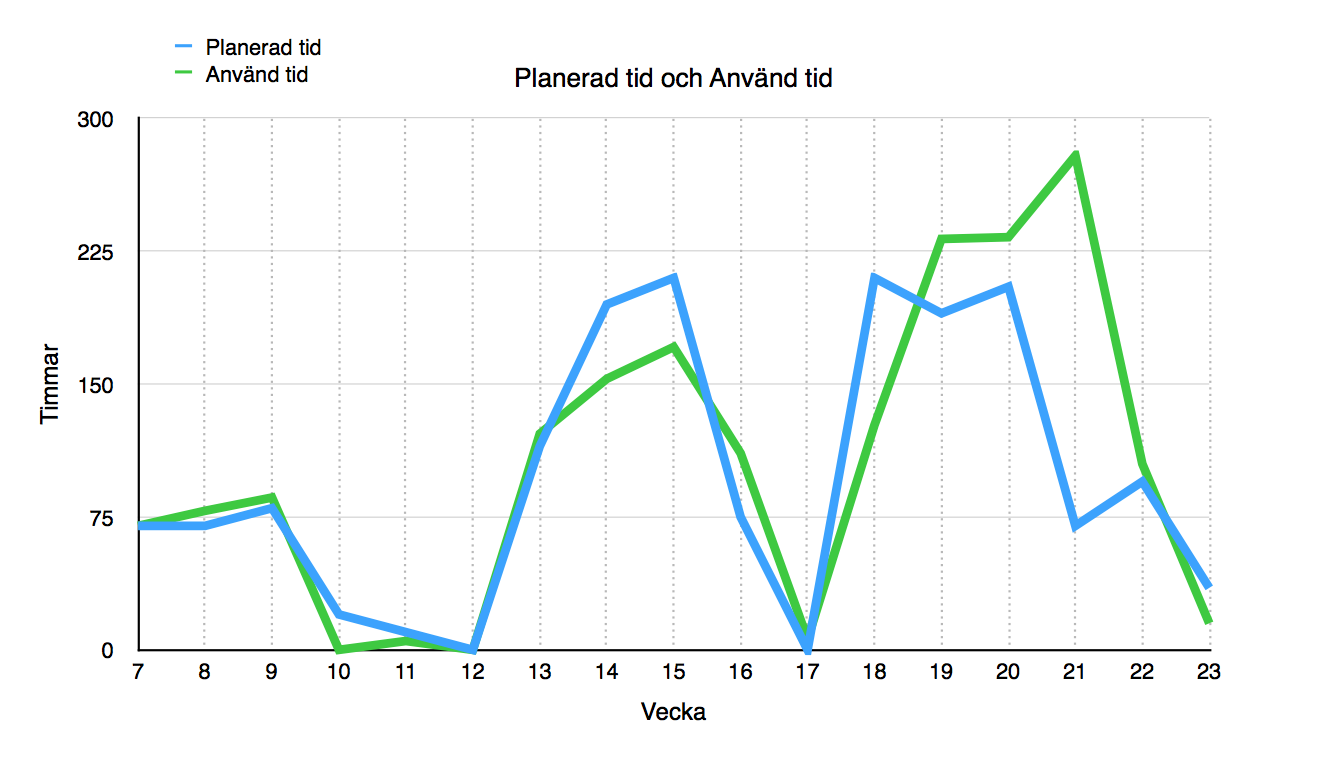
\includegraphics[keepaspectratio=true,scale=0.25]{tid.png}  %skala och filnamn. 
  \end{center}
  \caption{Diagram över planerad och använd tid} %figurtext.
  \label{fig:tid}
\end{figure}

\newpage

\section{Analys av arbete och problem}

\subsection{Vad hände under de olika faserna (bra/dåligt/orsak)}

\subsection{Hur använde vi projektmodellen}
Vi har genom hela projektet utgått från projektmodellen. Det som varit svårast med modellen är att försöka följa den första tidsplanen, istället har denna uppdaterats efterhand. I början av varje vecka har vi på ett mindre möte kollat över vilka aktiviteter som vi tycker borde ha mer/mindre tid under kommande vecka.

\subsection{Hur fungerade relationen med beställaren?}
Relation med beställaren har varit problemfri. Han svarar alltid snabbt på mail, verkar genuint intresserad och har alltid konstruktiv kritik att komma med.

\subsection{Hur fungerade relationen med handledaren?}
Ibland kunde vår handledare vara svår att nå. Det märktes tidigt att det krävdes en välformulerad och riktad fråga för att få ett bra svar, detta är självklart inga konstigheter och har istället hjälpt oss under projektet då en del fel löste sig genom att gruppen tänkte igenom frågor i detalj i förväg. I slutet av projektet var handledaren mycket lättare att nå och komma ofta förbi labbet för att kolla till sina grupper och deras status. Det märktes tydligt att handledaren var mycket kunnig.

\subsection{Tekniska framgångar/problem}

%Beskriv de 3 besvärligaste problemen som ni har haft under projektet. 
%Rangordna problemen där 1 är mest besvärlig i betydelsen tog längst tid att fixa.
%Beskriv för varje problem:
Hårdvarufel (4 parallella fel)

Bussproblem

Avståndsbestämning med hjälp av sensorer. 
%a. felets typ - ange t.ex.  hårdvarufel, mjukvarufel, systemintegrationsfel 
%b. kort beskrivning av felets symptom 
%c. kort beskrivning av felets orsak t.ex. logiskt fel i programmering, timing-fel, %glappkontakt, missförstånd av spec., felaktig design. 
%d. kort beskrivning av hur ni fixade felet. T.ex. hur ni fixade mjukvarubuggen, fick ny %hårdvara, virade om, gick runt problemet.
%e. ungefärlig skattning av hur mycket tid som ni ägnade åt felsökningen (dvs. tid som kunde tjänats in om felet inte hade uppstått)

\section{Måluppfyllelse}
Gruppen hade som initialt mål att leverera produkt med uppfyllda krav 1 mål samt att genomföra ett gott projekt. Detta tycker vi har uppfyllts även om kravbilden omförhandlats under projektets gång.
\subsection{Vad har uppnåtts?}
I dagsläget finns en robot som autonomt kartlägger ett slutet område med köksöar inuti. Den kan även detektera RFID-taggar, dock har vi haft problem med hårdvaran för denna och detta fungerar inte alltid. 

\subsection{Hur fungerade leveransen?}
Leveransen skedde genom ett möte med beställare där produkten demonstrerades genom en serie av körningar i olika typer av banor. Övriga funktioner såsom manuell styrning och kartlagring visades också upp. Kravlistan gicks igenom ett krav i taget och verifierades om målet var uppnått eller ej. I slutet av mötet tog beställare beslut om produkten var färdigställd. 
\subsection{Hur har studiesituationen påverkat projektet?}
Om möjligt skulle, inte bara för vår skull men även för andra examinatorer, projektkursen hållas enskilt utan övriga kurser parallellt. De flesta studenter prioriterat projektet över andra kurser, speciellt med tanke på hur många poäng kursen är värd.  

\section{Sammanfattning}
\subsection{De tre viktigaste erfarenheterna}
\subsection{Goda råd till de som ska utföra ett liknande projekt}
Det första rådet vi har till de som ska utföra ett liknande projekt är att planera noga och att fördela antalet arbetstimmar jämnt över hela projektettiden. En bra och tydlig planering är viktigt och kommer underlätta allt arbete. Att fördela arbetstimmarna jämnt över veckorna gör det lättare att lägga mer tid på andra kurser som läses parallellt med kandidatprojektet.

Det är också viktigt att lägga utveckling av bussprotokoll och buss i början av projektet, eftersom detta är något som kommer ta mycket tid att få till bra. Den kan med fördel testas mycket och med olika fall för att se att allt fungerar som det ska. Vi insåg i slutet av arbetet att vår buss inte var optimal, men då var det för sent för att göra något åt det.



\end{document}
